\documentclass[12pt]{article}
\usepackage{microtype}

% The preceding line is only needed to identify funding in the first footnote. If that is unneeded, please comment it out.
\usepackage{amsmath,amssymb,amsfonts}
\usepackage{algorithmic}
\usepackage{graphicx}
\usepackage{textcomp}
\usepackage{xcolor}
\usepackage{url}
\usepackage{listings}
\usepackage{courier}
\usepackage{xspace}
\usepackage{multirow}
\usepackage{colortbl}
\usepackage{blindtext}
\usepackage{float}
\usepackage{hyperref}
%\usepackage[font=scriptsize]{caption}
%\newcommand{\sd}[1]{\textbf{"\textsc{SD:}} \textit{#1}"}
%Dessin
\usepackage{tikz}
\usepackage{verbatim}
\usepackage{graphicx}
\usepackage[utf8]{inputenc}
\usepackage[english]{babel}
\usepackage{subfigure}
 \newboolean{showcomments}
\setboolean{showcomments}{true}
\ifthenelse{\boolean{showcomments}}
  {\newcommand{\bnote}[2]{
	\fbox{\bfseries\sffamily\scriptsize#1}
    {\sf\small$\blacktriangleright$\textit{#2}$\blacktriangleleft$}
    % \marginpar{\fbox{\bfseries\sffamily#1}}
   }
   \newcommand{\cvsversion}{\emph{\scriptsize$-$Id: macros.tex,v 1.1.1.1 2007/02/28 13:43:36 bergel Exp $-$}}
  }
  {\newcommand{\bnote}[2]{}
   \newcommand{\cvsversion}{}
  } 


\newcommand{\here}{\bnote{***}{CONTINUE HERE}}
\newcommand{\nb}[1]{\bnote{NB}{#1}}

\newcommand{\fix}[1]{\bnote{FIX}{#1}}
%%%% add your own macros 


\newcommand{\an}[1]{\bnote{Anne}{#1}}
\newcommand{\sd}[1]{\bnote{Stef}{#1}}
\newcommand{\ja}[1]{\bnote{Jannik}{#1}}
\newcommand{\md}[1]{\bnote{MD}{#1}}
\newcommand{\caro}[1]{\bnote{Caro}{#1}}
\newcommand{\jr}[1]{\bnote{JRe}{#1}}
\newcommand{\lf}[1]{\bnote{Luc}{#1}}
\newcommand{\gp}[1]{\bnote{Guille}{#1}}
\newcommand{\pt}[1]{\bnote{Pablo}{#1}}
\newcommand{\theo}[1]{\bnote{Theo}{#1}}
\newcommand{\spb}[1]{\bnote{Santiago}{#1}}
\newcommand{\bv}[1]{\bnote{Beno\^{i}t}{#1}}

\graphicspath{{figures/}}
%%% 


\newcommand{\figref}[1]{Figure~\ref{fig:#1}}
\newcommand{\figlabel}[1]{\label{fig:#1}}
\newcommand{\tabref}[1]{Table~\ref{tab:#1}}
\newcommand{\layout}[1]{#1}
\newcommand{\commented}[1]{}
\newcommand{\secref}[1]{Section \ref{sec:#1}}
\newcommand{\seclabel}[1]{\label{sec:#1}}

%\newcommand{\ct}[1]{\textsf{#1}}
\newcommand{\stCode}[1]{\textsf{#1}}
\newcommand{\stMethod}[1]{\textsf{#1}}
\newcommand{\sep}{\texttt{>>}\xspace}
\newcommand{\stAssoc}{\texttt{->}\xspace}

\newcommand{\stBar}{$\mid$}
\newcommand{\stSelector}{$\gg$}
\newcommand{\ret}{\^{}}
\newcommand{\msup}{$>$}
%\newcommand{\ret}{$\uparrow$\xspace}

\newcommand{\myparagraph}[1]{\noindent\textbf{#1.}}
\newcommand{\eg}{\emph{e.g.,}\xspace}
\newcommand{\ie}{\emph{i.e.,}\xspace}
\newcommand{\etal}{\emph{et al.,}\xspace}
\newcommand{\ct}[1]{{\textsf{#1}}\xspace}


\newenvironment{code}
    {\begin{alltt}\sffamily}
    {\end{alltt}\normalsize}

\newcommand{\defaultScale}{0.55}
\newcommand{\pic}[3]{
   \begin{figure}[h]
   \begin{center}
   \includegraphics[scale=\defaultScale]{#1}
   \caption{#2}
   \label{#3}
   \end{center}
   \end{figure}
}

\newcommand{\twocolumnpic}[3]{
   \begin{figure*}[!ht]
   \begin{center}
   \includegraphics[scale=\defaultScale]{#1}
   \caption{#2}
   \label{#3}
   \end{center}
   \end{figure*}}

\newcommand{\infe}{$<$}
\newcommand{\supe}{$\rightarrow$\xspace}
\newcommand{\di}{$\gg$\xspace}
\newcommand{\adhoc}{\textit{ad-hoc}\xspace}

\usepackage{url}            
\makeatletter
\def\url@leostyle{%
  \@ifundefined{selectfont}{\def\UrlFont{\sf}}{\def\UrlFont{\small\sffamily}}}
\makeatother
% Now actually use the newly defined style.
\urlstyle{leo}




 
\author{
        Bragagnolo, Santiago
}
\title{TP GIS4 - Anti-monopoly}
\date{\today}

 
\begin{document}
\maketitle
Cet exercise est basé sur un exercice proposé dans le cour de Paradigmes de programmation, à l'UTN, Argentine .

\section{Introduction}

\begin{figure}
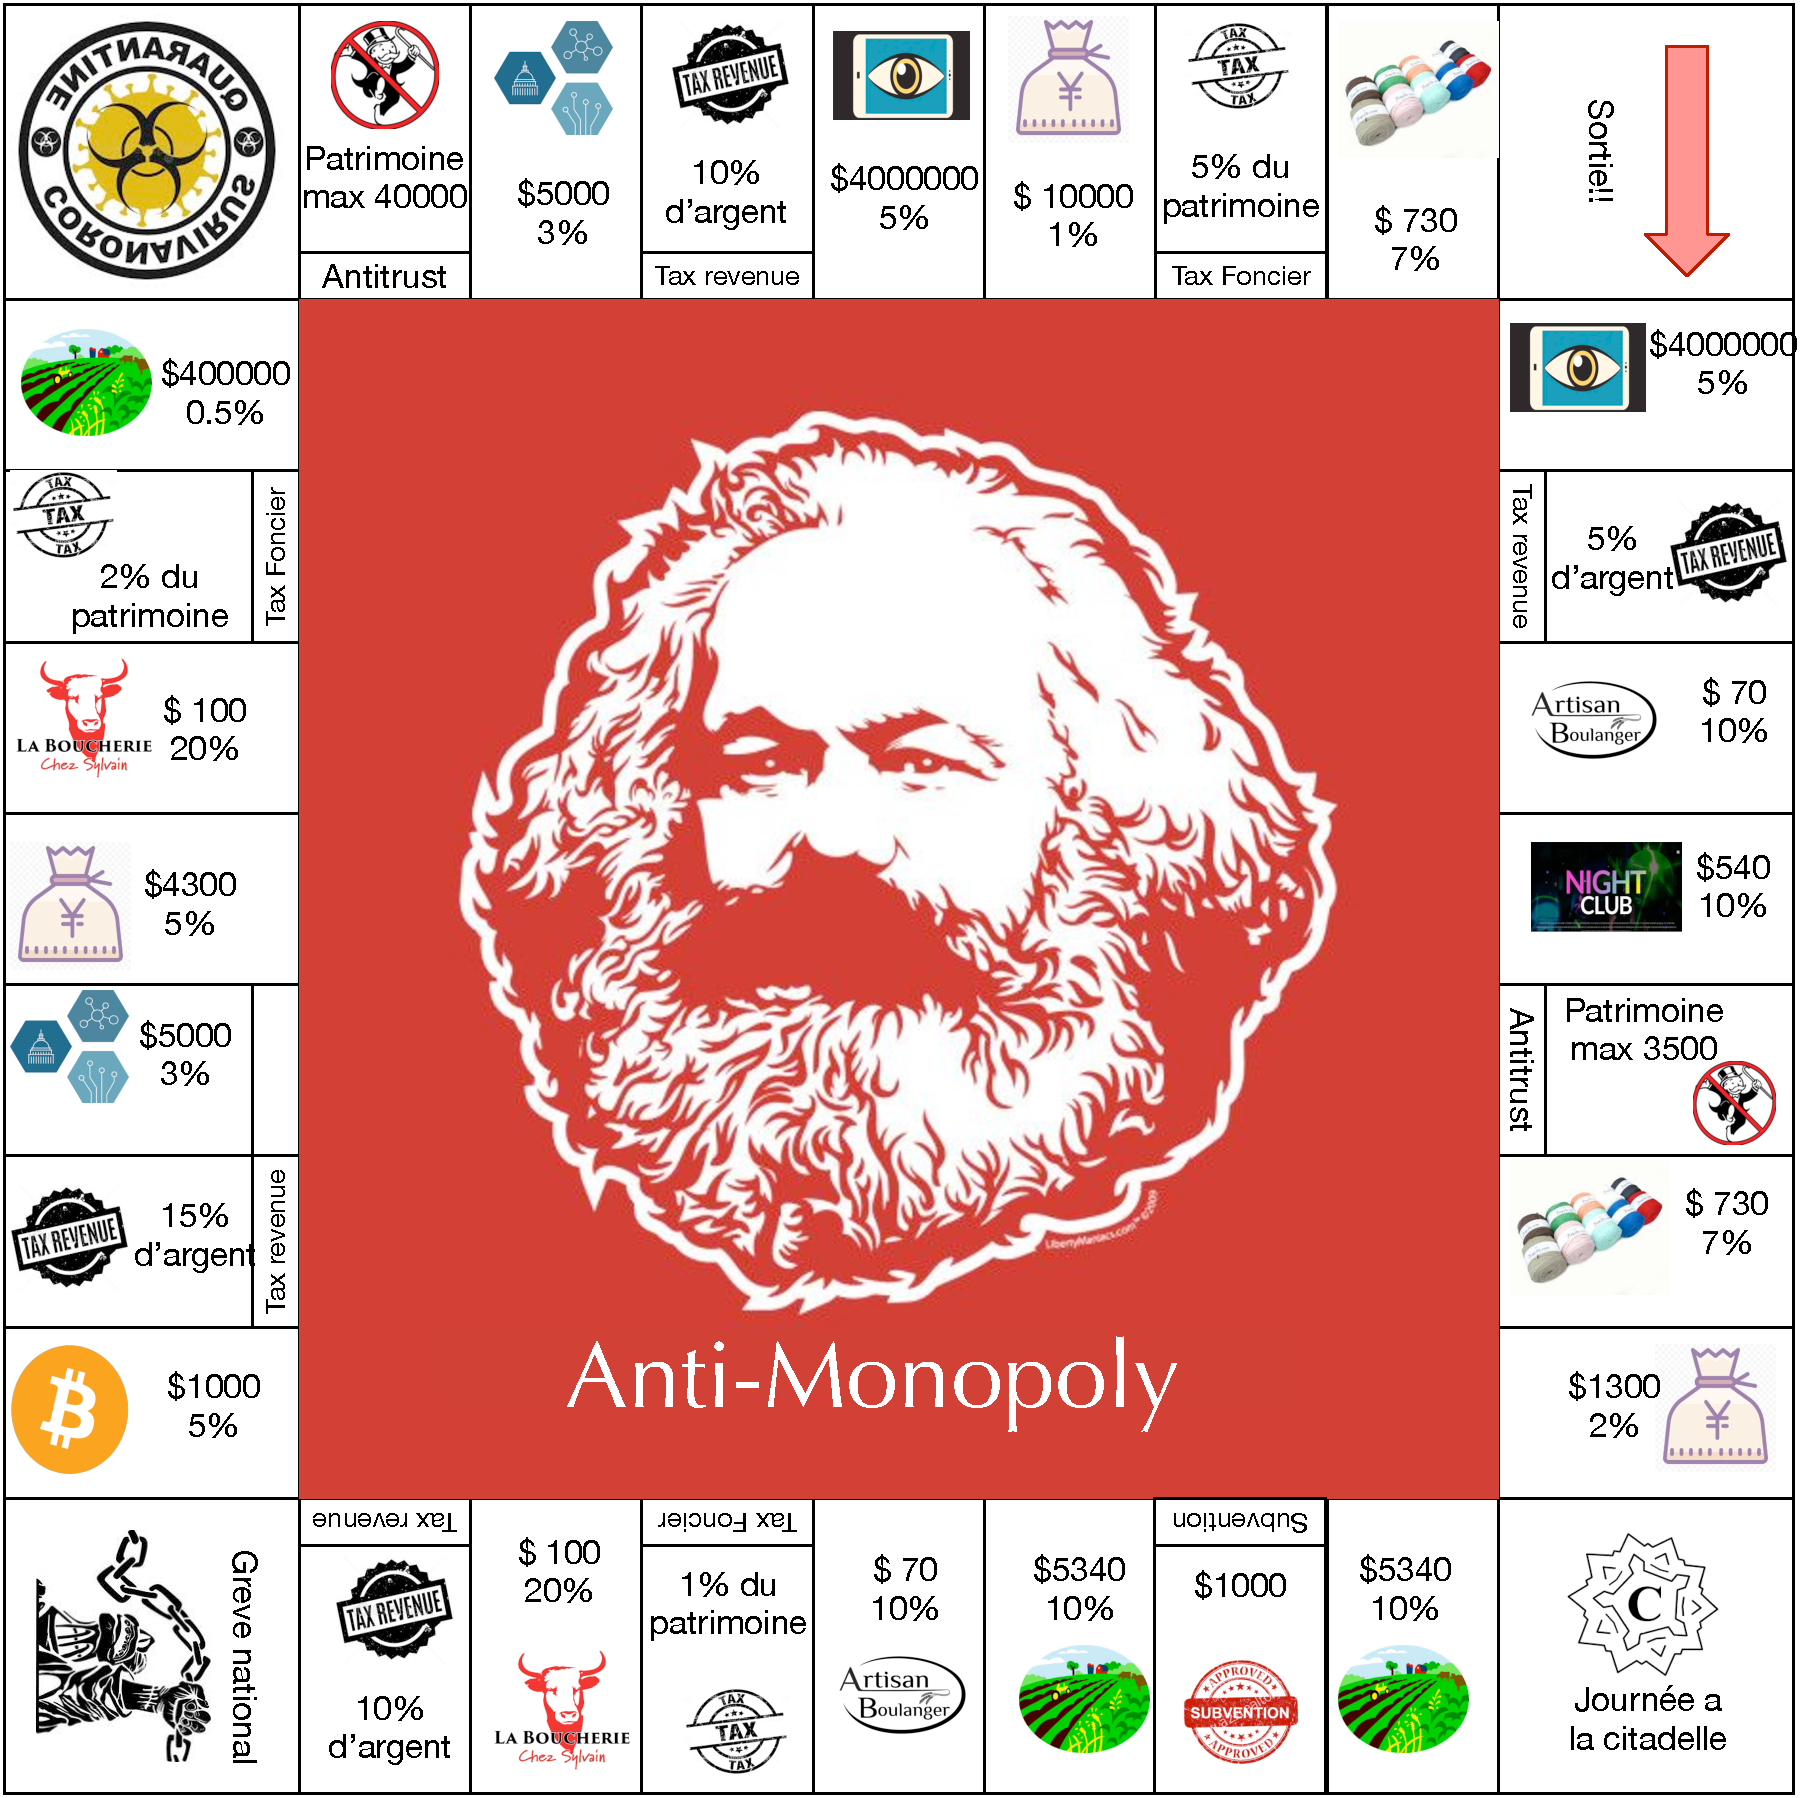
\includegraphics[width=15cm,height=15cm,keepaspectratio]{figures/board.pdf}
\caption{Exemple de tableau de jeu}
\end{figure}




Vous souhaitez implémenter un jeu de style Monopoly dans lequel les joueurs marchent sur un chemin où
ils doivent prendre des décisions d'investissement et faire certaines actions, afin d'augmenter votre
patrimoine. Attention à ne pas trop investir, parce que les lois antitrust peut vous obliger à
distribuer votre richesse.


\section{Caractéristiques du jeu}

    \subsection{Plateau du jeu}
    La Plateau est constitué d'un chemin circulaire composé d'un certain nombre de cases,
dans chacune desquelles il y a des indications. Il y a une case marquée "sortie" qui
indique le point de départ du jeu.

    \subsection{Des Joueurs}
    Il peut y avoir autant de joueurs que souhaité. Chaque joueur a un certain
montant initial d'argent. Au fur et à mesure que le jeu progresse, chacun des joueurs augmente
ou réduit son argent, selon les décisions d'investissement que chacun prend ou d'autres
circonstances qui vous viennent à l’esprit. Les capitaux propres d'un joueur correspondent à
son argent plus l'évaluation de tous les investissements qu'il a. Si un joueur perd tous ses capitaux qu'il ne peut pas continuer à jouer.

    
    \subsection{L'\'Etat}
    L'\'Etat est un acteur social dont la fonction principale est de réguler l'activité économique des
différents joueurs. Il a une certaine quantité de ressources financières.  L'Etat ne participe pas
au jeu en marchant sur le plateau, mais interagit avec tous les joueurs de différentes manières.

    \subsection{La dynamique de jeu}
    Initialement, tous les joueurs sont placés dans la case "sortie". À tour de rôle, chacun
    des joueurs lance un dé et avance d'où il se trouve d'autant de pas que l'indique le
    dé, arrivant ainsi à une nouvelle case. Là, le joueur doit suivre les instructions
    qui sont indiquées dans la case et prend les décisions économiques qu'il juge appropriées.
    De cette façon, tous les joueurs avancent à travers le plateau et font leur
    entreprise. Comme l'itinéraire est circulaire, il n'y a pas de point d'arrivée prédéterminé,
    raison pour laquelle ils continuent à tourner jusqu'à ce que l'on souhaite mettre fin au jeu.
    Le jeu est également terminé s'il reste un seul joueur ou si l'État échoue.
    
    \subsection{Case}
    
        
        Les cases peuvent être:
    \begin{itemize}
        \item Investissement: si l'investissement est disponible, 
        	le joueur décide s'il veut le prendre lui ou laissez passer. 
	Si l'investissement est déjà approprie par un autre joueur, qui tombe dans la boîte, 
	vous devez lui payer une somme d'argent proportion de la valeur de l'investissement.\an{pas compris cette phrase}\spb{TEXTE MODIFIE}.
        \item Loi antitrust: oblige le joueur à céder tous ses investissements
    qu'il possède et qui dépassent le maximum fixé par l'État. 
    Ces investissements reviennent à l'Etat, qui paie le joueur la moitié de leur prix. 
    Une fois entre les mains de l'état, ils sont disponibles pour les joueurs pour ce l'approprier. 
    \an{ca veut dire quoi qu'il reste a nouveau dispo}.\spb{TEXTE MODIFIE}
        \item  Bureau Finances publiques : oblige le joueur à payer à l'État un certain pourcentage de ses
    capitaux propres, au cas où il dépasserait une certaine valeur. Chaque taxe se calcule comme un percentage du patrimoine du joueur.
    Le percentage de chaque type d'impôt (impôt sur le revenu, impôt foncier personnel, etc.) est different. \an{pas compris la dernière phrase}\spb{TEXTE MODIFIE}
        \item Subvention: Le joueur reçoit de l'État le montant indiqué dans la case.
        \item Repos: C'est une case vide dans laquelle rien ne se passe. En particulier, la sortie
    en fait partie.
    \end{itemize}




    
    \begin{figure}
    \centering
    \subfigure[]{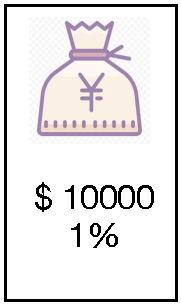
\includegraphics[width=2cm,height=2cm,keepaspectratio]{figures/investissement.pdf}} 
    \subfigure[]{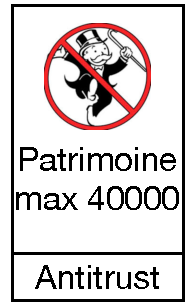
\includegraphics[width=2cm,height=2cm,keepaspectratio]{figures/antitrust.pdf}} 
    \subfigure[]{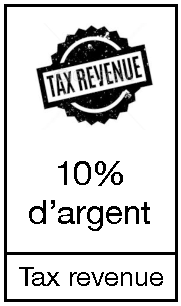
\includegraphics[width=2cm,height=2cm,keepaspectratio]{figures/taxe.pdf}}
      \subfigure[]{
\includegraphics[width=2cm,height=2cm,keepaspectratio]{figures/rienfaire.pdf}}

   
    \caption{(a) Investissment (b) Loi antitrust (c) finances publiques (d) subvention (e) activite non comercial}
    \label{fig:foobar}
\end{figure}



    \subsection{Investissements}
Les investissements sont le principal moyen pour les joueurs de gagner de l'argent. Initialement
l'\'Etat possède tous les investissement qui ont chacun un prix de référence, correspondant au
montant à payer par le joueur lorsqu'il tombe dans le cassier\an{c'est quoi la boite} et décide d'assumer ledit
investissement.
Chaque investissement génère un revenu calculé en pourcentage du prix de
référence, qui est chargé au joueur qui tombe dans le cassier \spb{TEXTE MODIFIE}\an{pas compris}. 
Prix et pourcentages de les bénéfices d'investissement sont complètement arbitraires.

    \subsection{Style des joueurs}

    Le fait qu'un joueur accepte ou non de conserver un investissement dépend en premier lieu 
    du fait qu'il a assez d'argent, mais aussi de son style de jeu. 
    Certains styles sont les suivants :
        \begin{itemize}
           \item Prudent: le joueur accepte l'investissement que s'il a moins d'un certain montant 
           d'investissements et que la valeur du nouvel investissement représente moins de 20 \% de ses
           actifs actuels.
           \item  Agressif: le joueur achete tout.
        \end{itemize}

    Finalement, si un joueur est obligé de se séparer de certains investissements, 
        il les choisit en fonction de son style de jeu:
        \begin{itemize}
            \item Prudent: ceux qui ont les prix les plus élevés.
            \item Agressif: le moins cher.
        \end{itemize}


        
\section{Exigences du projet}
Sur la base de l'approche générale du jeu, 
l'implémentation demandée doit comprendre :

\subsection{Définition initiale}
Créez un plateau de jeu avec plusieurs cases (au moins 10), des joueurs (au moins 2, un de
chaque style de jeu) et l'État. Tout définir prix, pourcentages, montants d’argent et
valeurs initiales nécessaires. 
Distribuer quantités et valeurs des cases d'une manière que vous considérez comme équilibrée.

\subsection{Simulation}

 Dans la method \texttt{main} effectuez les étapes suivantes, en choisissant arbitrairement la valeur des dés.
 \begin{itemize}
\item   Localisez tous les joueurs à la sortie.
\item    Demander à un joueur d'avancer un certain nombre de cases et de faire l'action correspondante.
\item    Vérifier la situation financière du joueur
\item    Faites jouer tous les joueurs en terminant un tour.
\item    Obtenez le classement des actifs des joueurs.
\item Simulez quelques tours jusqu'à ce qu'il ne reste qu'un joueur.
\end{itemize}


\subsection{Variantes}
Redémarrez le jeu en inventant les conditions initiales selon différentes
"Positions idéologiques", et voyez leur impact sur la simulation du jeu. Par
exemple :
\begin{itemize}
  \item NeoLiberal~: Certains joueurs avec beaucoup d'argent et d'autres avec peu, un état avec quelques
mesures antitrust légères.
  \item Socialiste~: Tous les joueurs avec le même argent de départ, beaucoup de taxes.
  \item Capitaliste~: tous les joueurs agressifs, pourcentages de profit élevés, plus élevés
ratio d'investissement.
  \item Progressiste : plus de joueurs, des lois antitrust strictes
combiné avec des subventions, des pourcentages de profit modérés.
  \item l'Europe après le Covid-19 : (au choix de chacun).
\end{itemize}
\end{document}

